Lo scopo di questa esperienza è la misurazione sperimentale delle caratteristiche (guadagno, frequenza di taglio, diagrammi di Bode) di un \textbf{filtro passa-basso} basato sull’operazionale LM1213. Il circuito è riportato in Figura \ref{fig:Circuit5}
Sono stati utilizzati i seguenti componenti:
\begin{itemize}
    \item Amplificatore operazionale 1213, codice ML1213
    \item Condensatore a film $C=100nF$
    \item Resistenza $R_1$, da 0.25W e valore da calcolare
    \item Resistenza $R_2$, da 0.25W e valore da calcolare
\end{itemize}
\begin{figure}[H]
    \centering
    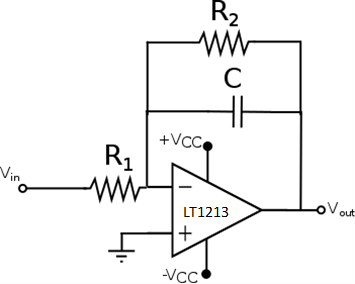
\includegraphics[width=0.45\linewidth]{images/Circuit5.png}
    \caption{Schema circuito}
    \label{fig:Circuit5}
\end{figure}
Il circuito è alimentato dalla tensione duale $\pm V_{CC}=\pm 10V$.
\subsection{PRELAB}
\subsubsection{Calcolare l'espressione della risposta in frequenza del filtro in Figura \ref{fig:Circuit5}}
Si ricavano le due impedenze: $Z_1=R_1$ e $Z_2=\frac{R_2}{sC}$. L'espressione della risposta in frequenza del filtro passa basso è
\begin{equation}
    G(s)=-\frac{Z_2}{Z_1}=-\frac{R_2}{R_1}\frac{1}{1+sCR_2}
\end{equation}
\subsubsection{Definizione dei valori di $R_1,R_2$}
E' richiesto di determinare i valori di $R_1,R_2$ affinché il filtro passa-basso ha guadagno in bassa frequenza pari a 0dB e frequenza di taglio pari a 1kHz. Dalla funzione di trasferimento del filtro si ottiene l'espressione del guadagno a bassa frequenza
\begin{equation}
    A_0=-\frac{R_2}{R_1}=0dB\implies \frac{R_2}{R_1}=1\implies R_2=R_1
\end{equation}
Dalla frequenza di taglio si ricava il valore delle resistenze
\begin{equation}
    F=\frac{1}{2\pi R_2C}=1kHz\implies R_2=R_1=\frac{1}{2\pi CF}\approx1.6k\Omega
\end{equation}
\subsubsection{Tracciare il diagramma di Bode del modulo e della fase del filtro}
\begin{figure}[H]
    \centering
    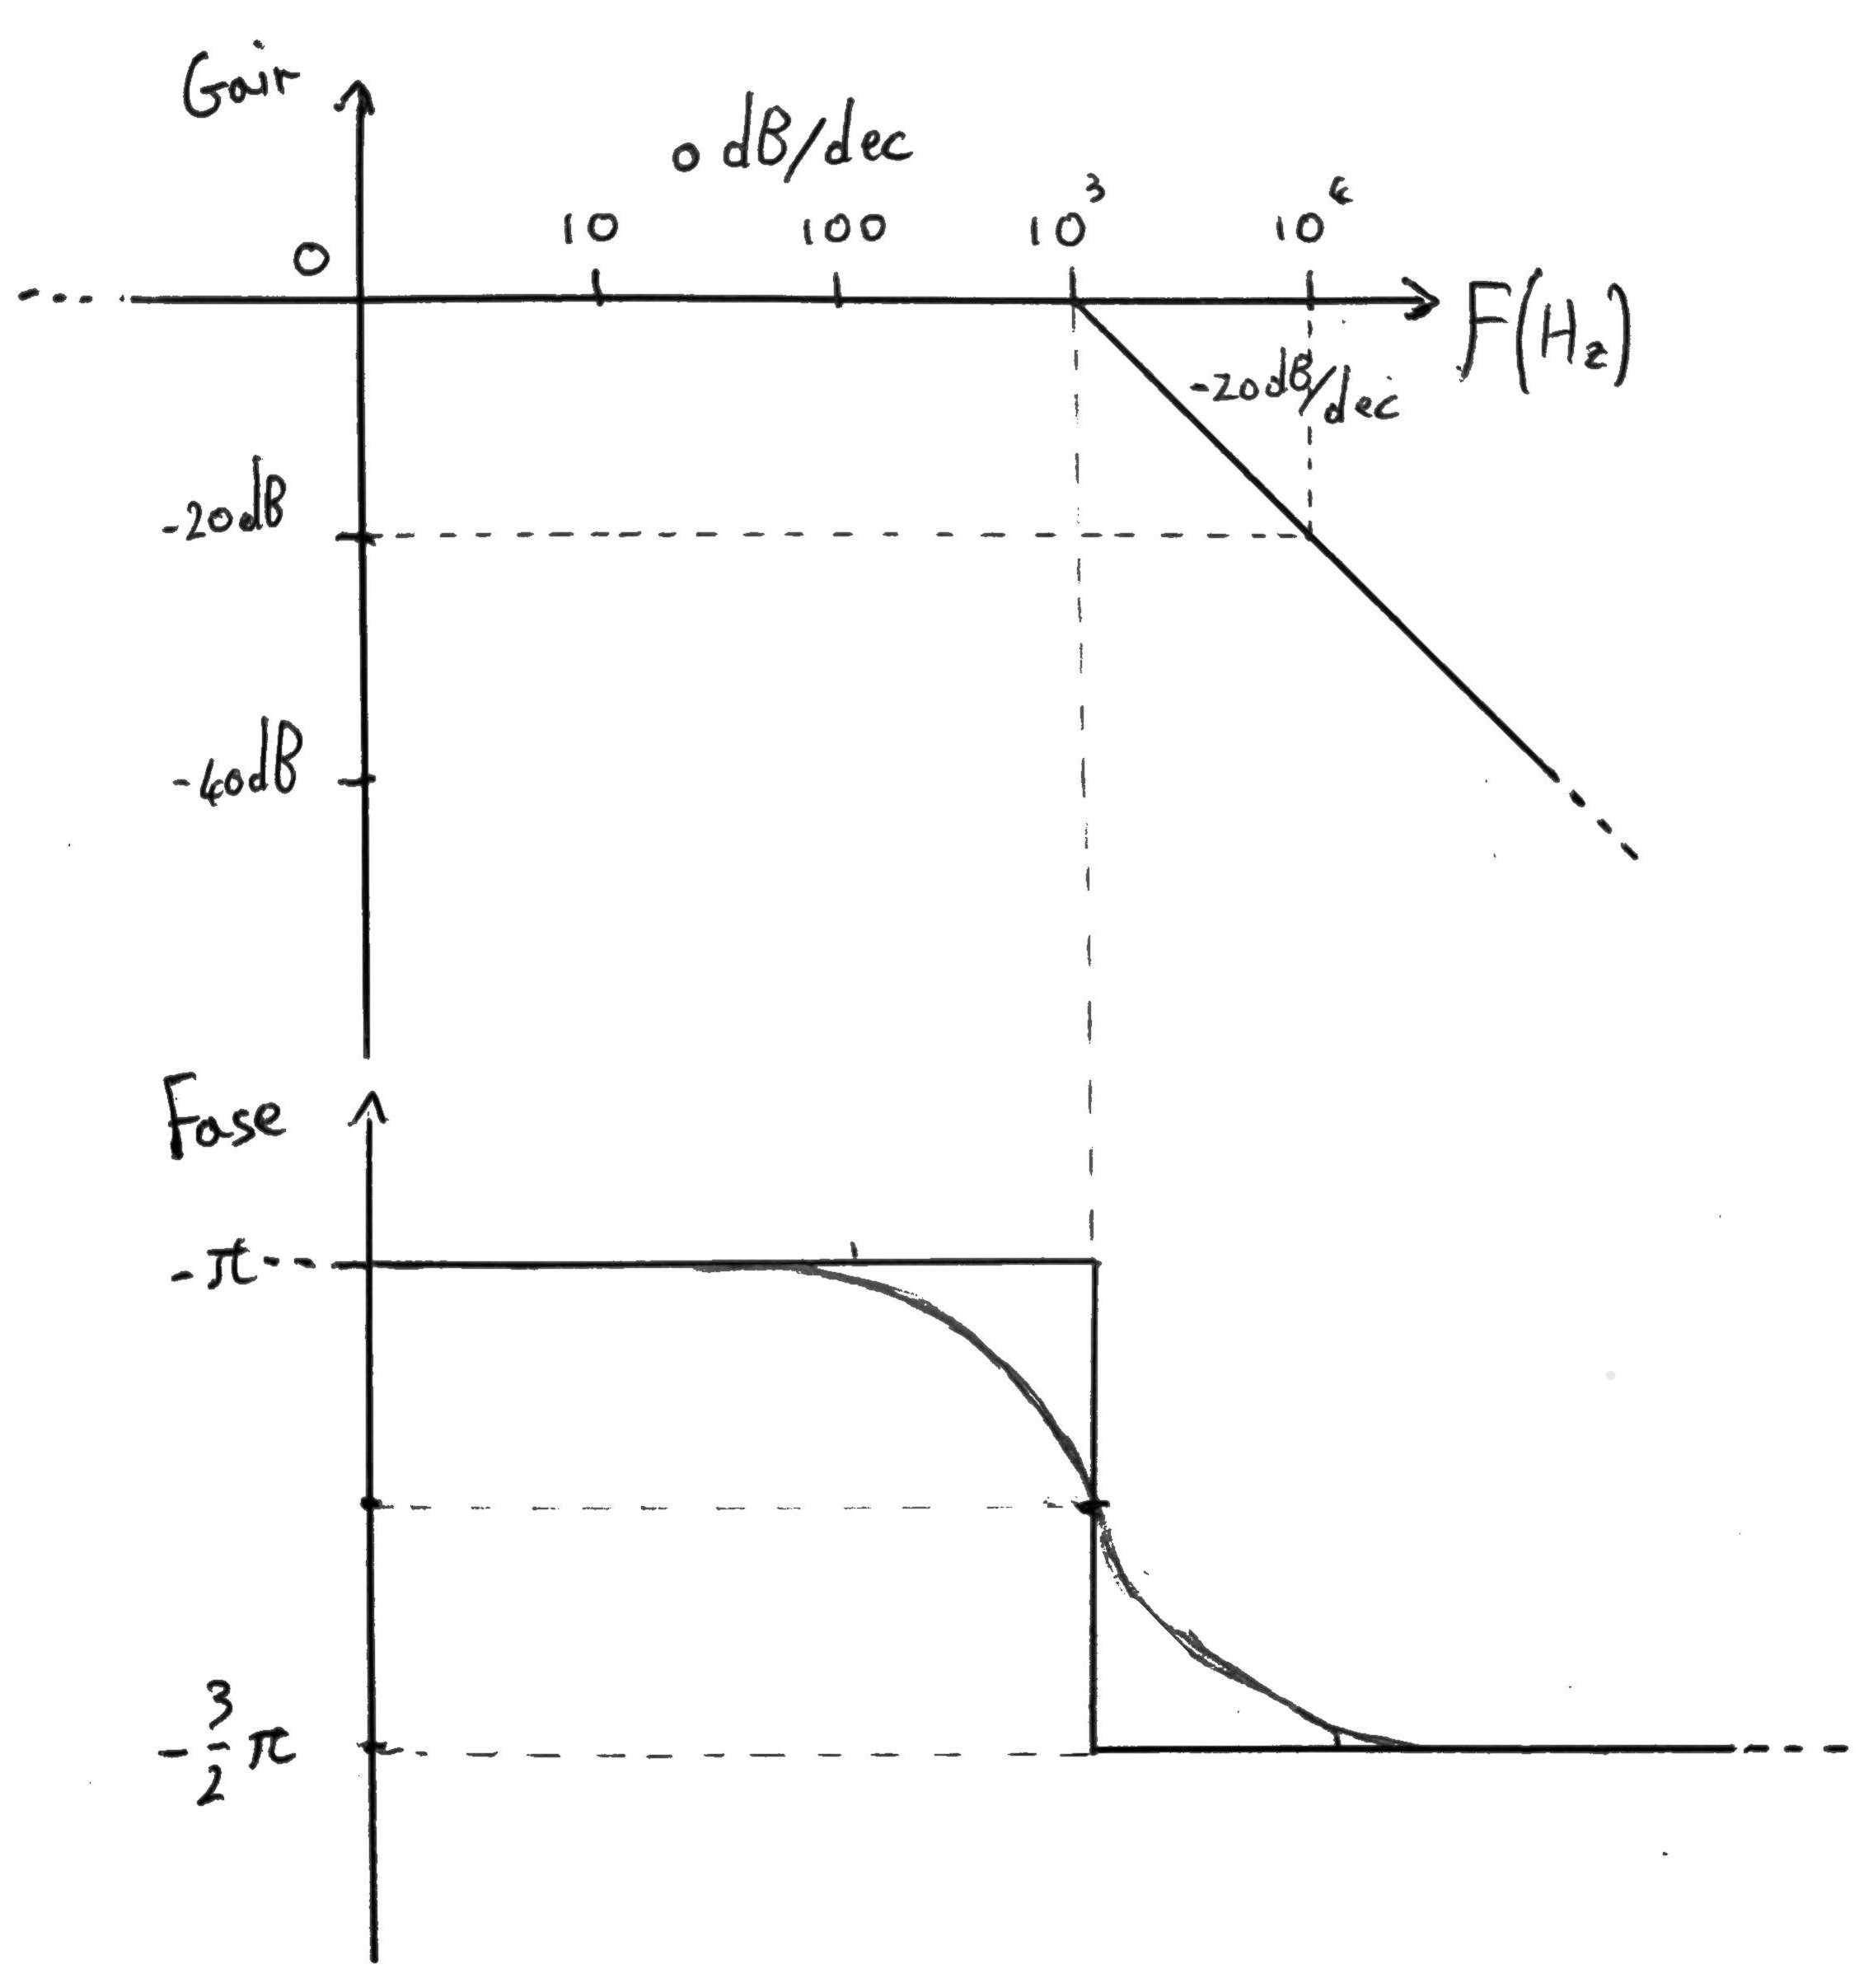
\includegraphics[width=0.8\linewidth]{images/BodeMan.jpeg}
    \caption{Diagramma di bode}
    \label{fig:BodeMan}
\end{figure}
\clearpage
\subsection{Simulazione SPICE con LTspice\textregistered\xspace}
Dopo aver riportato lo schematico in Figura \ref{fig:Circuit5} su LTspice\textregistered\xspace, è stata svolta l'analisi in frequenza con la direttiva \texttt{.ac dec 100 10 100k} da 10 Hz a 100kHz, il circuito SPICE è mostrato in Figura \ref{fig:SpiceES5}.
\begin{figure}[H]
    \centering
    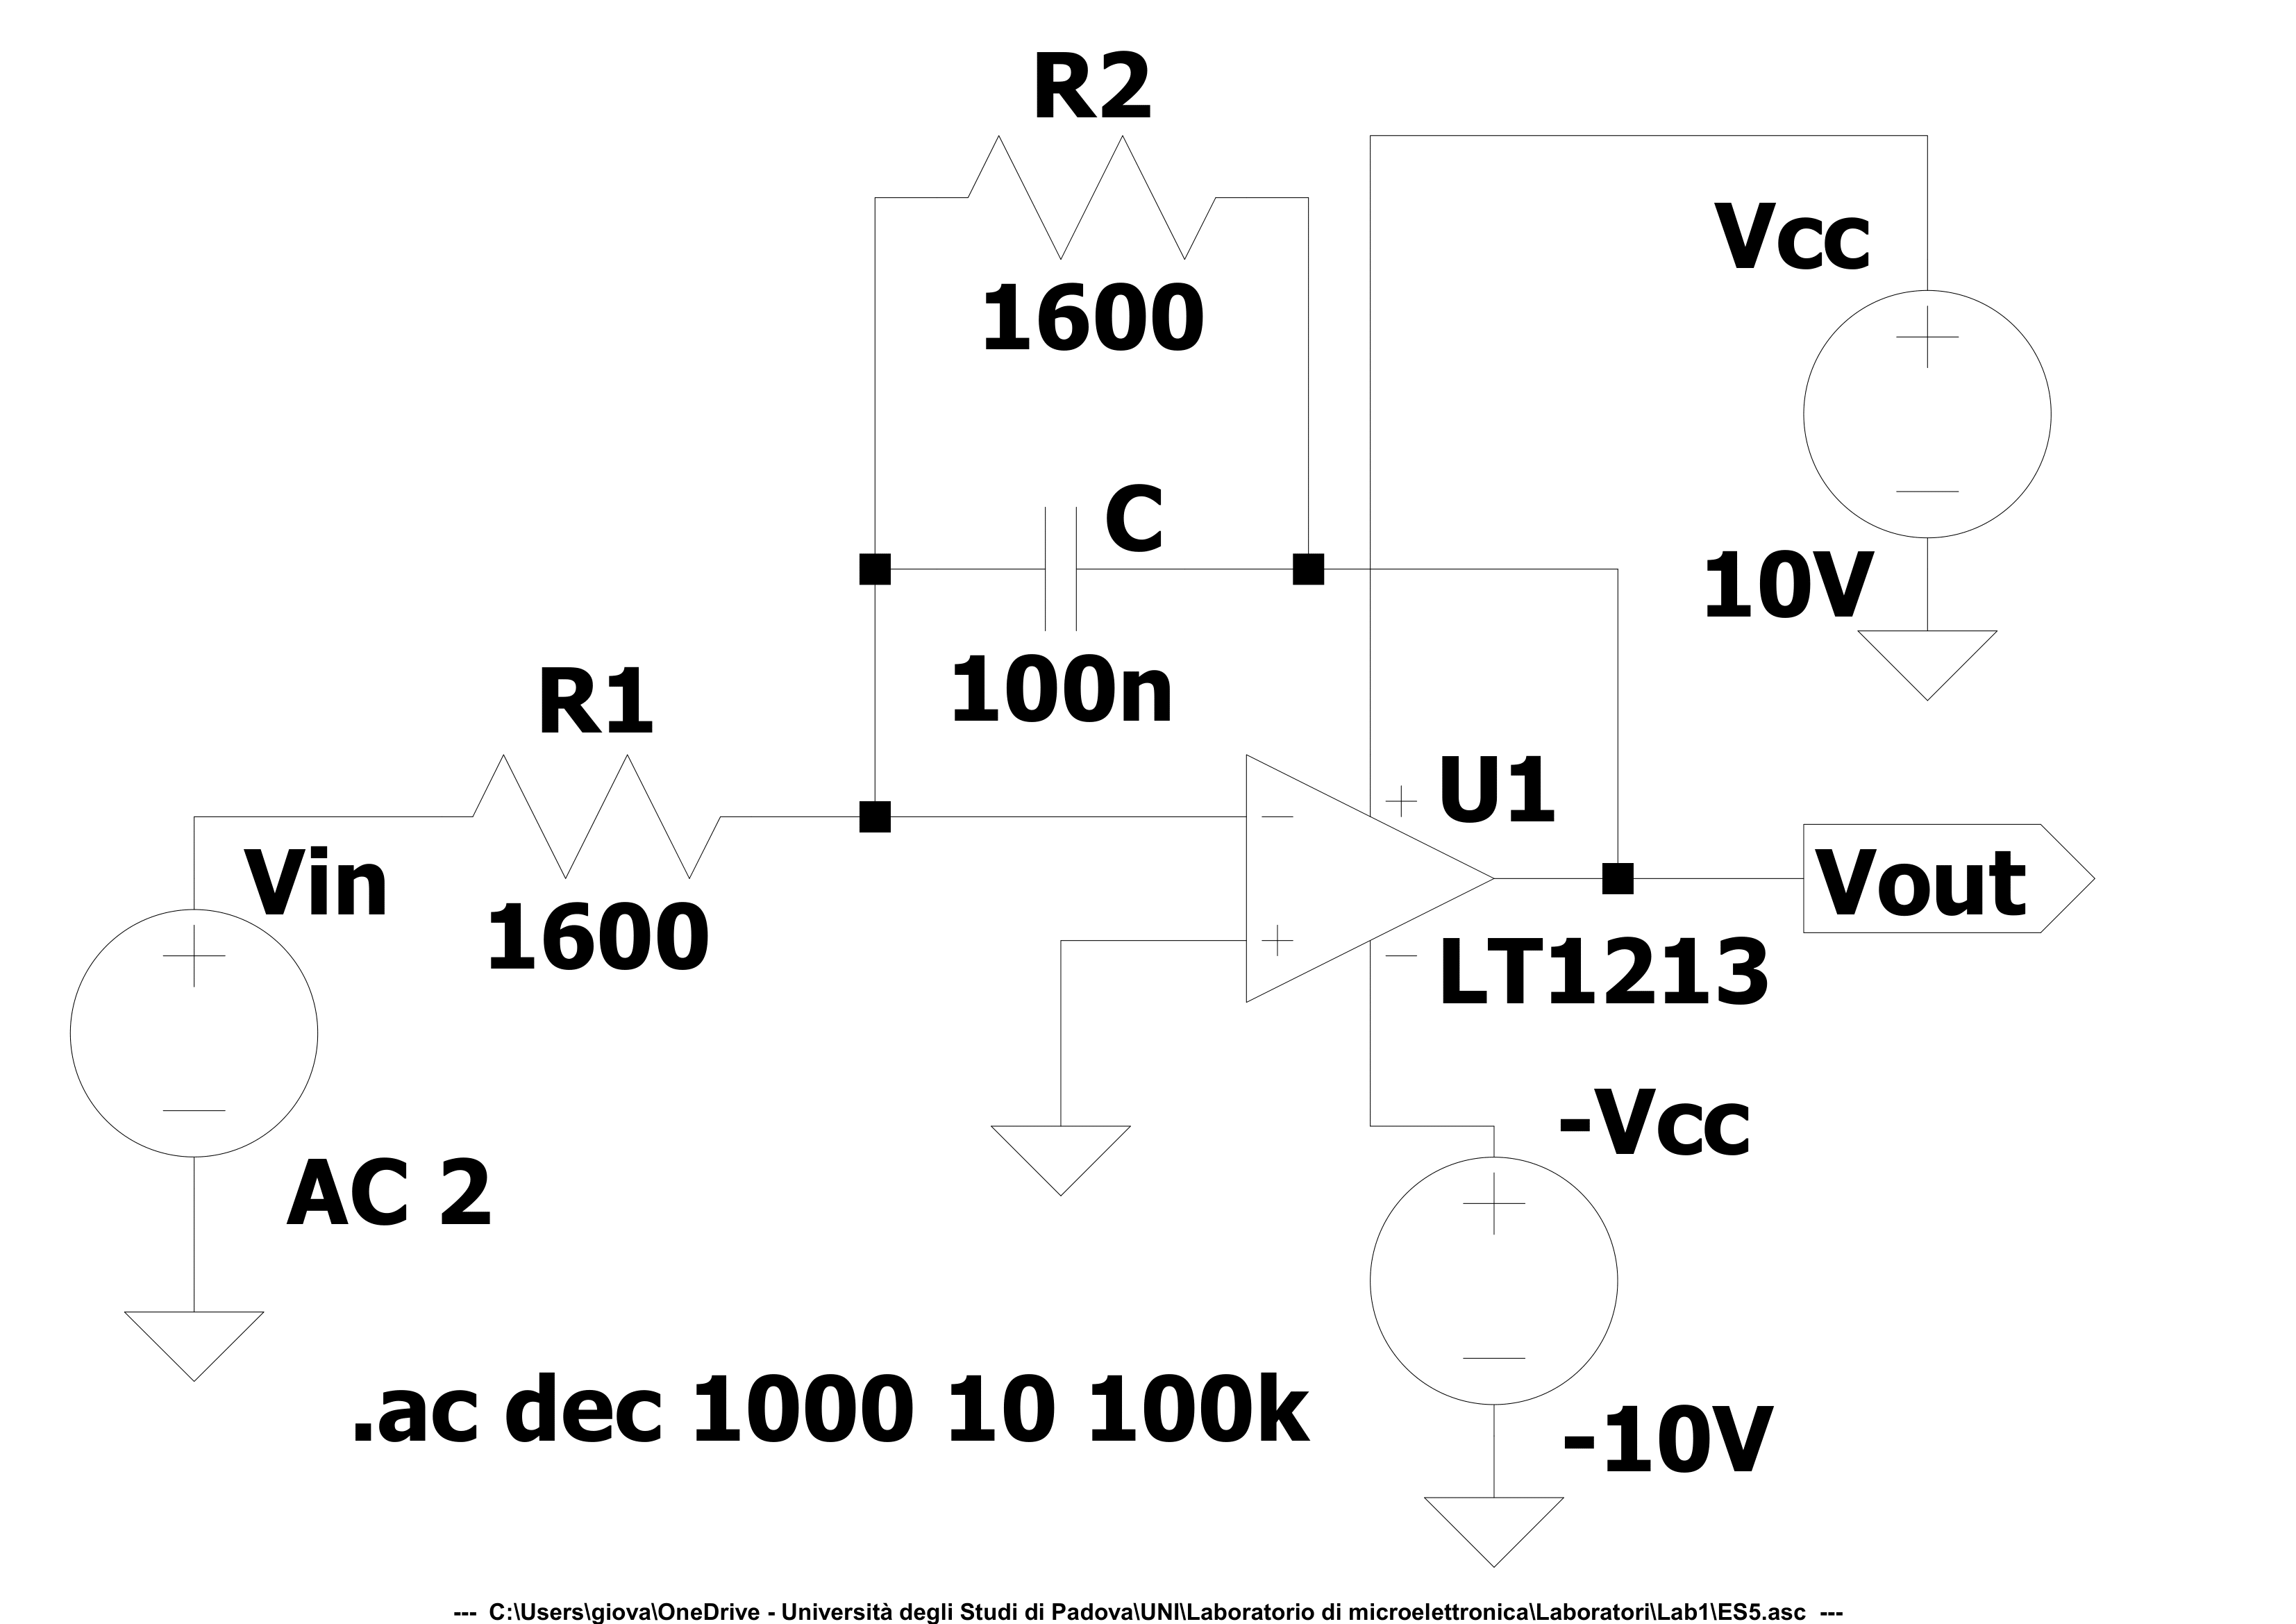
\includegraphics[width=0.55\linewidth]{images/ES5-1.png}
    \caption{Circuito SPICE}
    \label{fig:SpiceES5}
\end{figure}
L'analisi in frequenza ha prodotto il seguente diagramma di Bode del modulo e della fase, riportato in figura \ref{fig:SpiceBodeES5}
\begin{figure}[H]
    \centering
    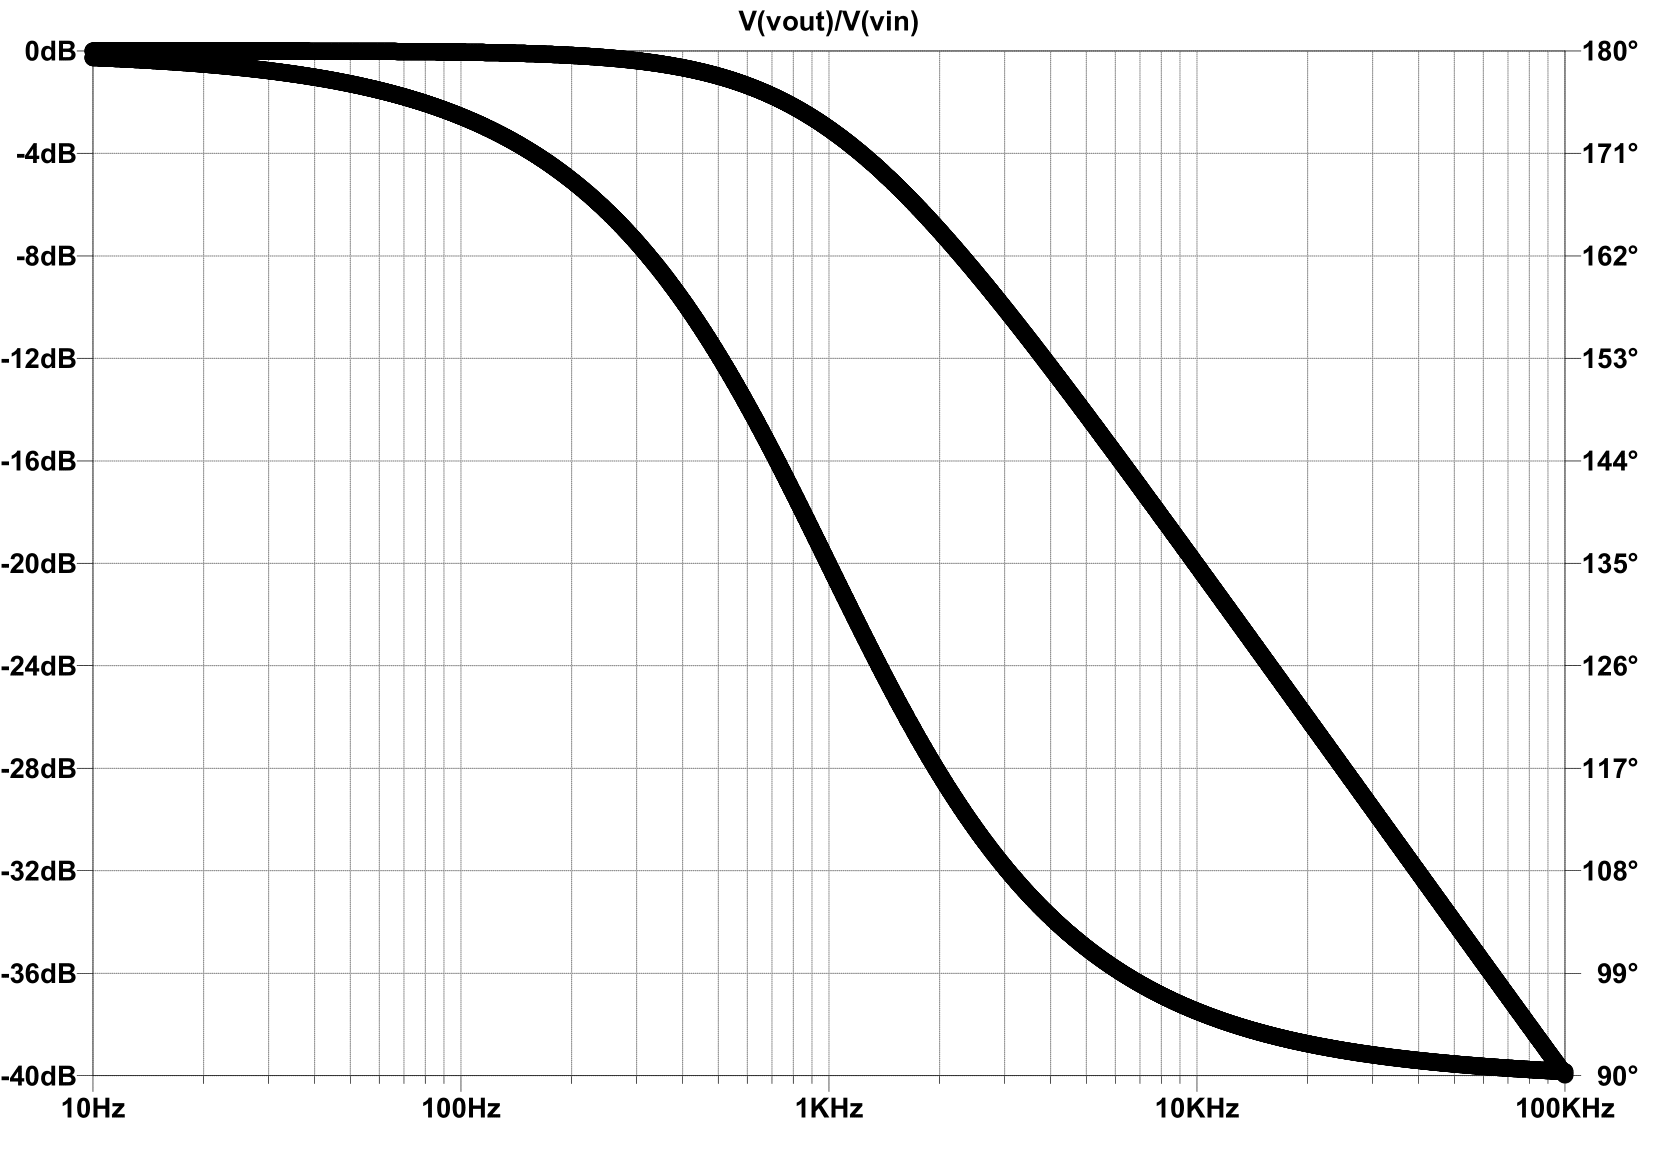
\includegraphics[width=0.6\linewidth]{images/Plot_ES5-1.png}
    \caption{Diagramma di Bode generato da LTspice\textregistered}
    \label{fig:SpiceBodeES5}
\end{figure}
Come si può notare dal diagramma, in corrispondenza della frequenza di taglio a $1kHz$ si ha che la pendenza passa da $0dB/dec$ a $-20dB/dec$, come si prevedeva in base ai calcoli svolti.\\\\
Per ricavare il guadagno in bassa frequenza si può utilizzare la direttiva SPICE \texttt{.tf v(Vout) Vin} che ci fornisce 
\begin{equation}
    A_{BF}=\frac{V_{out}}{Vin}=-0.999998 V/V = 20\log_{10}{(\left|-0.999998\right|)}=-0.00001737...\approx0dB
\end{equation}
Dal grafico si nota che alla frequenza di $1kHz$ il guadagno arriva a -3dB
\subsection{Risultati sperimentali}
Dopo aver montato il circuito il Figura \ref{fig:Circuit5} e averlo connesso al generatore di segnale si è alimentato il circuito con una tensione duale di $\pm V_{CC}=\pm10V$. 
\begin{figure}[H]
    \centering
    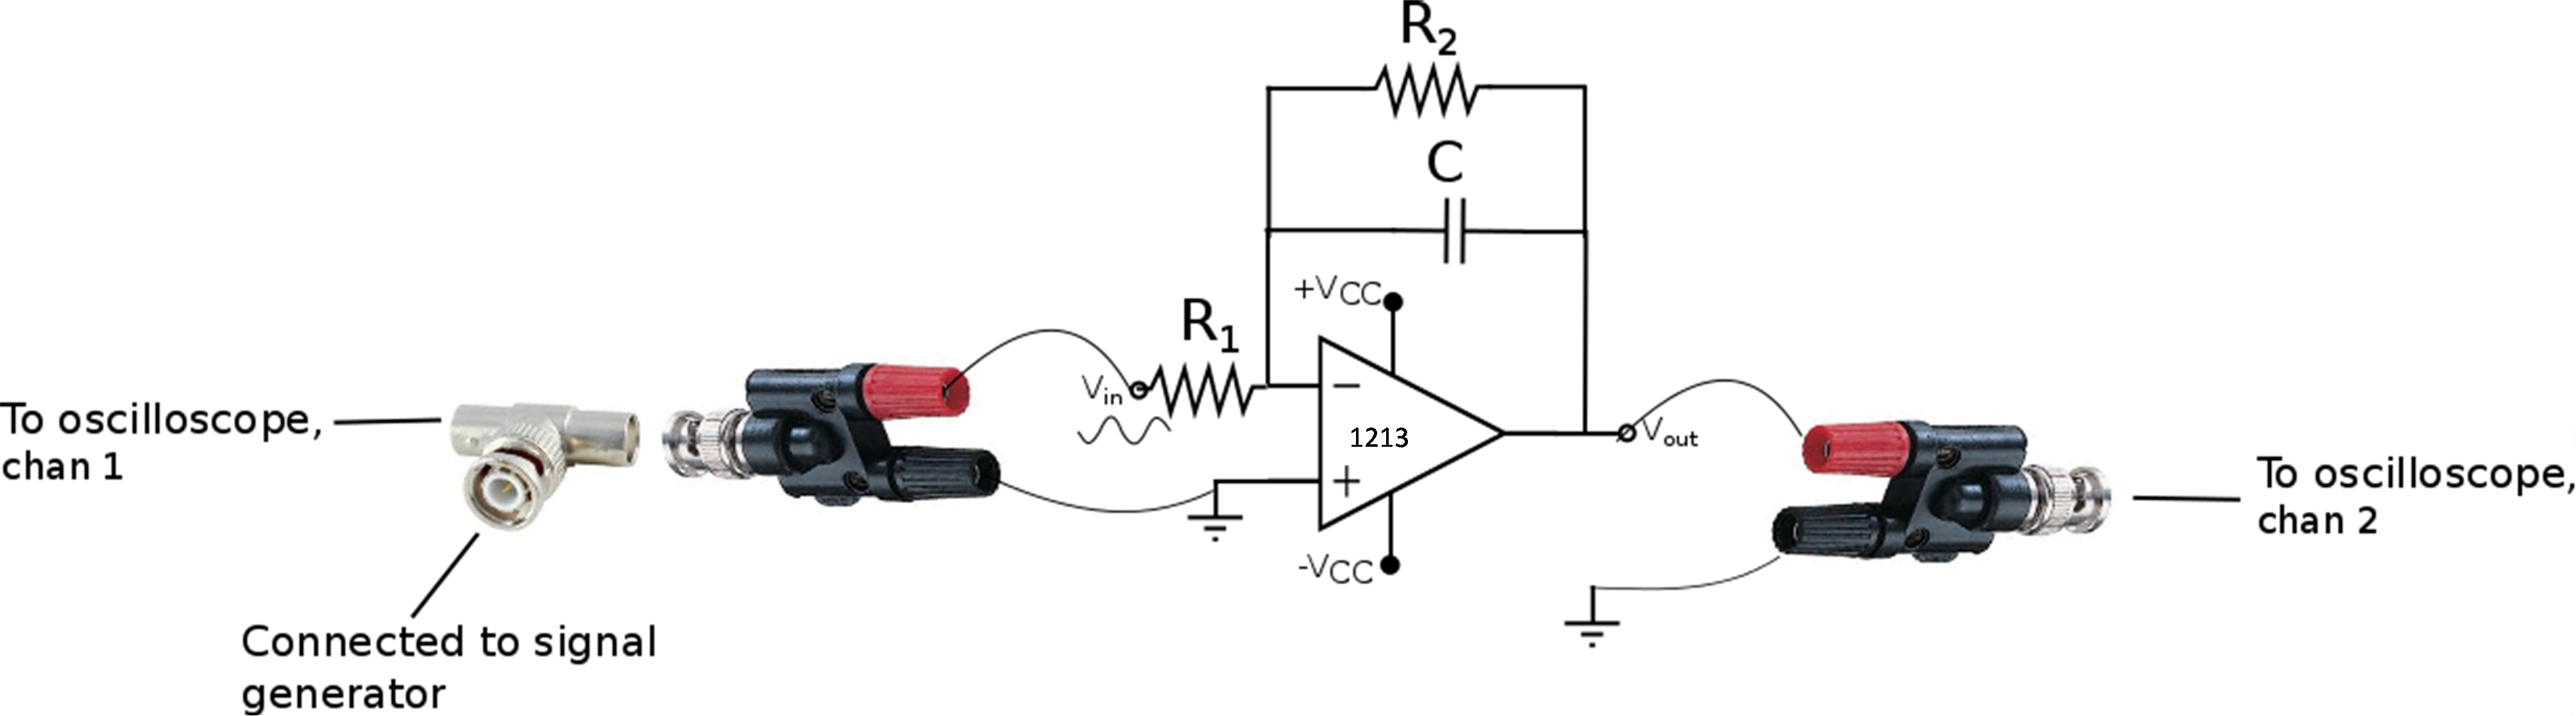
\includegraphics[width=0.8\linewidth]{images/LabCircuit5.png}
    \caption{Schema di collegamento del circuito}
    \label{fig:LabCircuit5}
\end{figure}
Il generatore di segnale è stato impostato in modo da applicare in ingresso al circuito il seguente segnale:
\begin{itemize}
    \item Forma d'onda: sinusoidale
    \item Ampiezza: $2V_{PP}$
    \item Frequenza: 10 Hz
    \item Offset: 0V
\end{itemize}
Successivamente si sono svolte le misure e il calcolo del guadagno in bassa frequenza del circuito con i valori di tensione picco-picco ricavati dall'oscilloscopio
\begin{equation}
    \text{Guadagno BF} = \frac{V_{out}}{V_{in}} = 1.00195 =_{dB} 0.016921 dB
\end{equation}
Si è poi concluso misurando il diagramma di Bode del modulo e della fase del filtro in Figura \ref{fig:Circuit5}, effettuando le misure a diversi valori di frequenza. I risultati sono riportati in Tabella \ref{tab:Ris5}
\begin{table}[H]
    \centering
    \begin{tabular}{||c|c|c|c|c||}
    \hline
       Frequenza (Hz)  & $V_{outPP}$ (V) & Guadagno & Guadagno (dB) & Fase  \\\hline\hline
       10 & 1.93125 V & 1.0095 & 0.01692 & -179.42° \\\hline
       30 & 1.93125 V & 1.0095 & 0.01692 & -178.3° \\\hline
       50 & 1.92 V & 0.9961 & -0.03394 & -177.16° \\\hline
       100 & 1.92 V & 0.9961 & -0.03394 & -174.2° \\\hline
       300 & 1.8375 V & 0.9533 & -0.4154 & -162.3° \\\hline
       500 & 1.68825 V & 0.8759 & -1.1509 & -151.5° \\\hline
       1000 &  1.303 V & 0.6760 & -3.401 & -133.3° \\\hline
       3000 & 552.4 mV & 0.2897 & -10.761 & -105.3° \\\hline
       5000 & 358.31 mV & 0.1859 & -14.614 & -99.3° \\\hline
       10000 & 76.67 mV & 0.03977 & -28 & ----° \\\hline
       
    \end{tabular}
    \caption{Risultati}
    \label{tab:Ris5}
\end{table}
I dati rilevati in laboratorio sono stati elaborati con l'ausilio di MATLAB\textregistered\xspace e riportati nei diagrammi di Bode del modulo e della fase, rispettivamente riportati in Figura \ref{fig:BodeModEXP} e \ref{fig:BodeFasEXP}.
\begin{figure}[H]
    \centering
    \begin{minipage}{.5\textwidth}
      \centering
      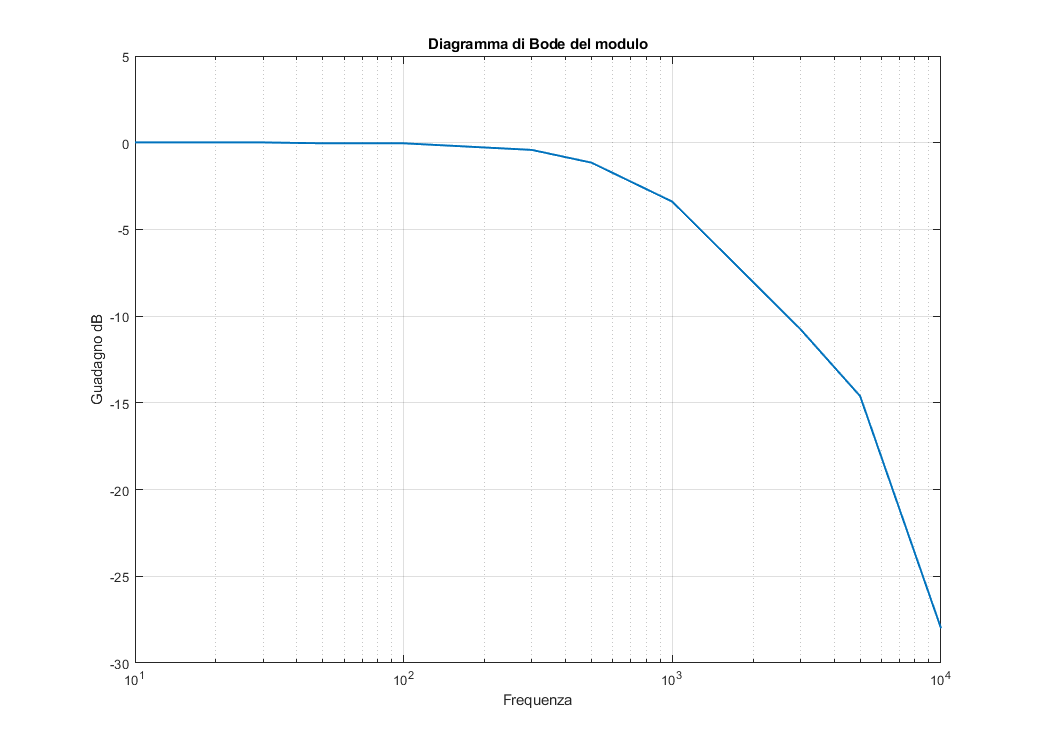
\includegraphics[width=\linewidth]{images/BodeModEXP.png}
      \captionof{figure}{Diagramma di Bode del modulo}
      \label{fig:BodeModEXP}
    \end{minipage}%
    \begin{minipage}{.5\textwidth}
      \centering
      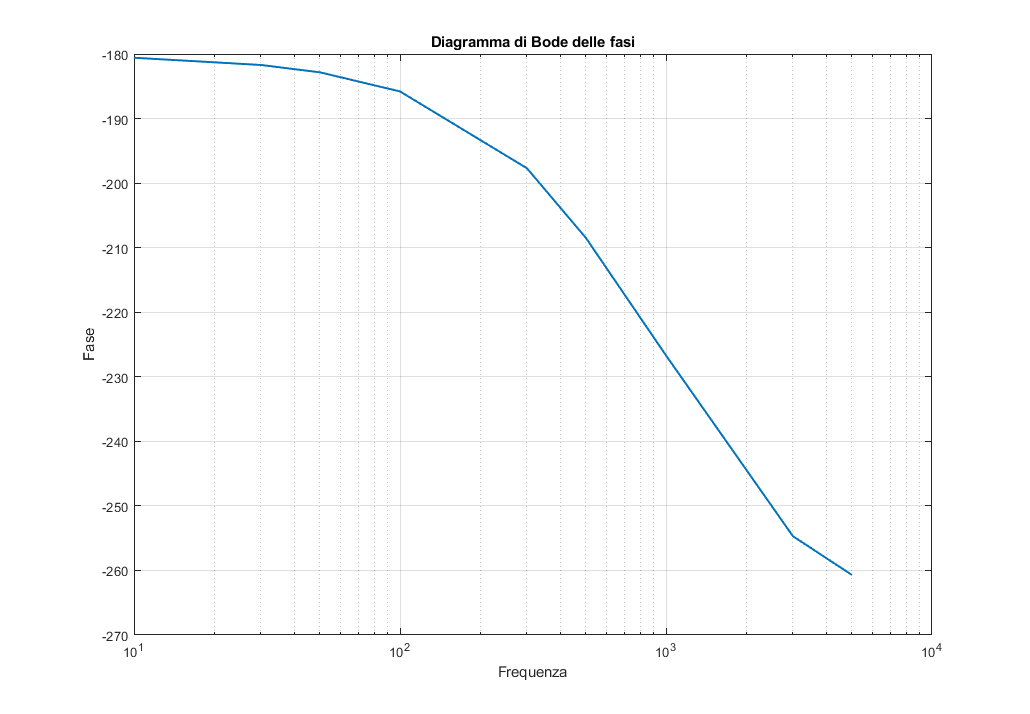
\includegraphics[width=\linewidth]{images/BodeFasEXP.png}
      \captionof{figure}{Diagramma di Bode delle fasi}
      \label{fig:BodeFasEXP}
    \end{minipage}
\end{figure}
\begin{comment}
\begin{figure}[H]
   \centering
    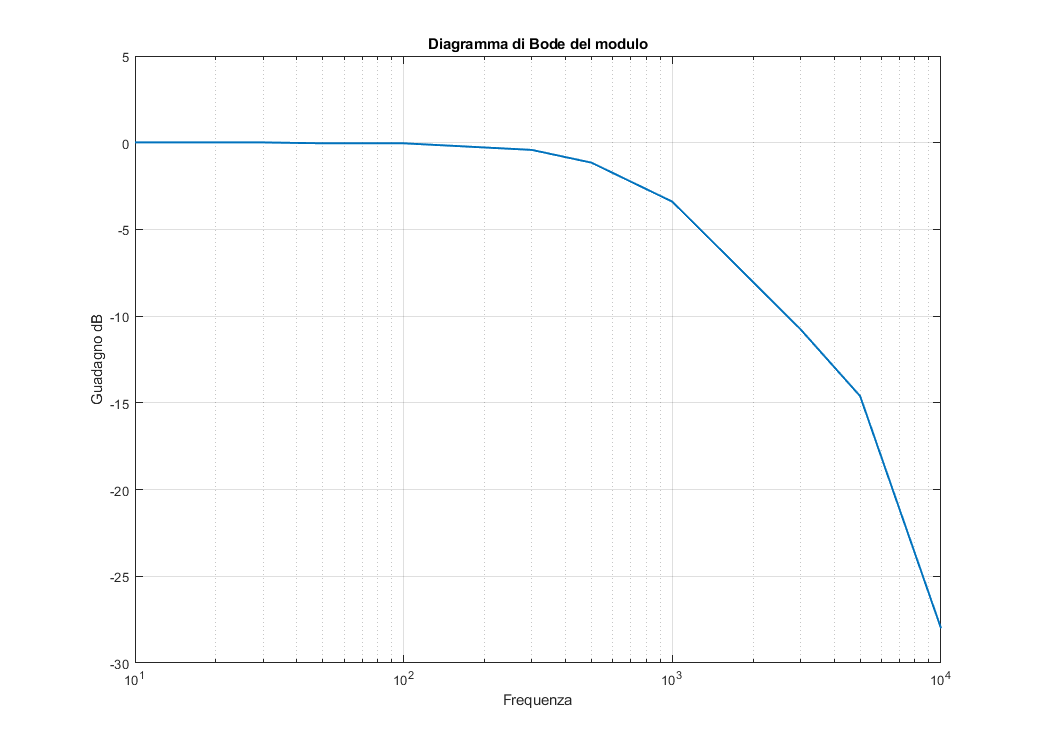
\includegraphics[width=0.7\linewidth]{images/BodeModEXP.png}
    \caption{Diagramma di Bode del modulo}
    \label{fig:BodeModEXP}
\end{figure}
\begin{figure}[H]
    \centering
    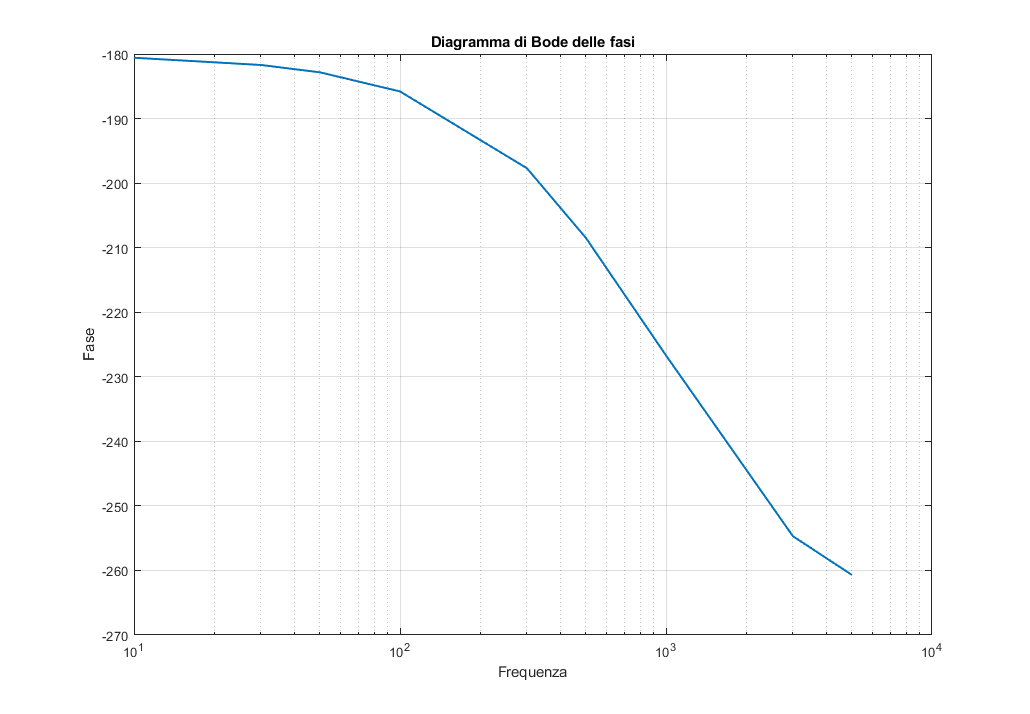
\includegraphics[width=0.7\linewidth]{images/BodeFasEXP.png}
    \caption{Diagramma di Bode delle fasi}
    \label{fig:BodeFasEXP}
\end{figure}
\end{comment}
\subsection{Conclusioni}
Confrontando l'andamento dei diagrammi di Bode misurati, in Figura \ref{fig:BodeModEXP} e \ref{fig:BodeFasEXP}, con quelli simulati mediante LTspice \textregistered\xspace si può notare che l'andamento è concorde per quanto riguarda il diagramma dei moduli.\\\\
Per quanto riguarda il diagramma della fase il valore misurato alla frequenza di 10kHz non aveva un valore stabile sull'oscilloscopio, per tanto, al fine di non incorrere in errori di misura esso è stato trascurato.